\documentclass{llncs}

\usepackage{amssymb}
\usepackage{tikz}

\usetikzlibrary{arrows,automata}

\begin{document}

\title{Poset Paper}
\author{Bow-yaw Wang\inst{1} \and Chih-chen Yuan\inst{2}}
\institute{Academia Sinica, Taiwan\\ \and
National Taiwan Normal University, Taiwan\\}
\maketitle

\begin{abstract}
hello world
\end{abstract}

\section{Introduction}
Intro part here

\section{Preliminaries}
% emph what's defined

A partial order is a binary relation that is reflexive, antisymmetric, and transitive. A partially ordered set or poset is a binary structure $\mathcal{P} = (\mathrm{\Omega}, \leq)$ where the \emph{universe} $\mathrm{\Omega}$ is a set and $\leq$ is a partial order on $\mathrm{\Omega}$; we refer to members of $\mathrm{\Omega}$ as elements of $\mathcal{P}$ and, where specificity is desired, to $\mathrm{\Omega}$ as $\mathrm{\Omega}_{\mathcal{P}}$ and $\leq$ as $\leq_{\mathcal{P}}$.

\begin{example}
    For the following definition, consider the poset $\mathcal{P}$ over $\{a,b,c,d\}$ with $a \leq b$; $a \leq c$; $a \leq d$; $b \leq d$; and $c \leq d$. Figure \ref{figure:posetp} represents $\mathcal{P}$ with a graph $(\mathrm{V},\mathrm{E}) = (\mathrm{\Omega},\prec)$.
    % change to text ;graph describ
    \label{example:posetp}
\end{example}

\begin{figure}
\centering
\vspace{1cm}
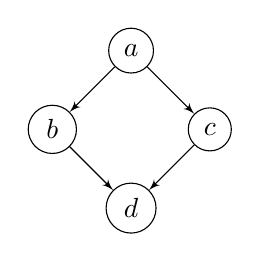
\begin{tikzpicture}
    [
    vertex/.style={circle,draw,minimum size=1.5em},
    edge/.style={->,> = latex'}
    ]
\node[vertex] (1) at (1,2) {$a$};
\node[vertex] (2) at (0,1) {$b$};
\node[vertex] (3) at (2,1) {$c$};
\node[vertex] (4) at (1,0) {$d$};
\draw[edge] (1) -- (2);
\draw[edge] (1) -- (3);
\draw[edge] (2) -- (4);
\draw[edge] (3) -- (4);
\end{tikzpicture}
\caption{Graph representation of Example~\ref{example:posetp}.}
\label{figure:posetp}
\end{figure}

The cover relation $\prec$ of a poset $\mathcal{P}$ is the transitive reduction of the order relation; it describes the case of immediate successor: for $x, y \in \mathcal{P}$, $x \prec y$ iff $x \leq y \wedge \not\exists z \in \mathcal{P}, x \leq z \wedge z \leq y$. For \textit{Example 1}, the cover relation includes $a \prec b$; $a \prec c$; $b \prec d$; and $c \prec d$. Note that $(a, d)$ is absent in $\prec$.

In addition, we describe the case of incomparability in a poset $\mathcal{P}$ with $\parallel$: for $x, y \in \mathcal{P}$, $x \parallel y$ iff $x \not\leq y \wedge y \not\leq x$. For \textit{Example 1}, there is $b \parallel c$.

%A Hasse diagram $\mathcal{H}$ sums up a poset $\mathcal{P} = (\mathrm{\Omega}, \leq)$ with a directed acyclic graph $\mathcal{H} = (\mathrm{V},\mathrm{E})$, where the nodes $\mathrm{V} = \mathrm{\Omega}$ and the edges $\mathrm{E} = \prec$. *Figure 1* shows the Hasse diagram of *Example 1*.

\begin{example}
    For the following definition, consider the poset $\mathcal{L}$ over $\{a,b,c,d\}$ with $a \leq b$; $a \leq c$; $a \leq d$; $b \leq c$; $b \leq d$; and $c \leq d$. \textbf{Fig.2} represents $\mathcal{L}$ with a graph $(\mathrm{V},\mathrm{E}) = (\mathrm{\Omega},\prec)$.
\end{example}

\begin{figure}
\centering
\vspace{1cm}
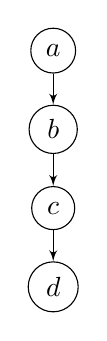
\begin{tikzpicture}
    [
    vertex/.style={circle,draw,minimum size=1.5em},
    edge/.style={->,> = latex'}
    ]
\node[vertex] (1) at (0,3) {$a$};
\node[vertex] (2) at (0,2) {$b$};
\node[vertex] (3) at (0,1) {$c$};
\node[vertex] (4) at (0,0) {$d$};
\draw[edge] (1) -- (2);
\draw[edge] (2) -- (3);
\draw[edge] (3) -- (4);
\end{tikzpicture}
\caption{Graph representation of \textit{Example 2}.}
\end{figure}

A partial order that is also total is called a linear order; every pair of elements are comparable in a linear order. Note that the graph representation of a linear order is a chain. For simplicity, we represent a linear order in string form. For \textit{Example 2}, we write $abcd$.

\section{Swap Graph}
intro and cite linearization???
%1 summary
%2 informal swap

% remove
\begin{theorem}
    (Szpilrajn Theorem) For a partial order $\mathcal{P}$, there exists a linear order $\mathcal{L}$ that extends $\mathcal{P}$; that is, $\leq_{\mathcal{P}} \subseteq \leq_{\mathcal{L}}$.
\end{theorem}

For a poset $\mathcal{P}$, a linear order $\mathcal{L}$ that extends $\mathcal{P}$ is called a linear extension or linearization of $\mathcal{P}$, and we write $\mathcal{P} \sqsubseteq \mathcal{L}$ iff $\mathcal{L}$ is a linearization of $\mathcal{P}$. For example, for $\mathcal{P}$ from \textit{Example 1} and $\mathcal{L}$ from \textit{Example 2}, $\mathcal{P} \sqsubseteq \mathcal{L}$. Note that a linearization of a poset is equivalent to a topological sort of the graph representation of that poset???.

The set of all linearizations of $\mathcal{P}$ is denoted $\mathcal{L}(\mathcal{P})$. We shall consider it the language of a poset[Appendix]. By \textbf{Theorem 1}, $\mathcal{L}(\mathcal{P}) \neq \emptyset$. For $\mathcal{P}$ from \textit{Example 1}, $\mathcal{L}(\mathcal{P}) = \{abcd, acbd\}$.

intro and cite swap graph/adjacent transposition g???

The swap relation $\leftrightarrow$ describes the case of ``off by one swap'' between linear orders with shared universe: for linear orders $\mathcal{L}_{1}, \mathcal{L}_{2}$ and $x, y \in \mathrm{\Omega}$, $\mathcal{L}_{1} \leftrightarrow_{x, y} \mathcal{L}_{2}$ iff $\leq_{\mathcal{L}_{1}} \cap \leq_{\mathcal{L}_{2}} = \leq_{\mathcal{L}_{1}} \cup \leq_{\mathcal{L}_{2}} - \{(x,y),(y,x)\}$. For example, $abcd \leftrightarrow_{b, c} acbd$. Note that $\leftrightarrow$ is symmetric.

%define on upsilon
The swap graph $\mathcal{G}(\mathcal{P})$ of a poset $\mathcal{P}$ is constructed as the undirected graph $(\mathrm{V},\mathrm{E})$ such that $\mathrm{V} = \mathcal{L}(\mathcal{P})$ and $\mathrm{E} = \{(\mathcal{L}_{1}, \mathcal{L}_{2}) | \exists x,y \in \mathcal{P}, \mathcal{L}_{1} \leftrightarrow_{x, y} \mathcal{L}_{2}\}$. \textbf{Fig.3} shows the swap graph $\mathcal{G}(\mathcal{P})$ of $\mathcal{P}$ from \textit{Example 1}.

%if one poset then connected (informal)

\begin{figure}
\centering
\vspace{1cm}
\begin{tikzpicture}
    [
    vertex/.style={circle,draw,minimum size=1.5em},
    edge/.style={grow right sep=1cm}
    ]
\node[vertex] (1) at (0,0) {$abcd$};
\node[vertex] (2) at (2,0) {$acbd$};
\draw[edge] (1) -- (2);
\end{tikzpicture}
\caption{Swap graph of $\mathcal{P}$ from \textit{Example 1}.}
\end{figure}

\begin{theorem}
    (Pruesse? and Ruskey) For a poset $\mathcal{P}$, the swap graph $\mathcal{G}(\mathcal{P})$ is connected. cite???
\end{theorem}

That's it? should we move the swap things to motivations?

\section{Problem Definition?or Poset Cover Problem}
intro pcp; intro converse of lin; intro trivial non-max solution? intro np completeness?

The poset cover problem is: given a set of linearizations $\Upsilon$, find a set of posets $\mathcal{C}$, called a cover, such that $\Upsilon = \bigcup_{P \in C} \mathcal{L}(P)$ and that $|\mathcal{C}|$ is minimal.

\begin{theorem}
    insulating barrier method where?
\end{theorem}

\section{SAT Encoding Part}
We use the boolean logic of z3 SMT solver from MS research. Since poset is connected, by contraposition, we can first divide and conquer on connected components of the swap graph, by solving each component individually.

We then check with incrementing number of posets to find the minimal number of posets to cover each component. We first encode the axioms of posets; namely, reflexivity, antisymmetry, and transitivity. Next, we encode the extension constraint with contraposition from input linearizations to reduce the number of variables. Finally, we encode the non-extension constraint with negation of extension constraint on the insulating barrier.

\section{Exp Part}
NOTE: how do i put graph here?

\section{Conclusions}

\section{References}
NOTE: how to use list?

\section{Appendix}

\begin{theorem}
    Permutations and Nerode
\end{theorem}

\begin{theorem}
    (Corollary of Szpilrajn extension theorem) For a partial order $\leq$, $\leq = \bigcap_{< \in \mathcal{E}(\leq)} <$.
\end{theorem}

\begin{theorem}
    (Heath and Nema) If $x \parallel y$ for $\leq$ and there is $< \in \mathcal{E}(\leq)$ such that $x \prec y$ for $<$, then there is $<' \in \mathcal{E}(\leq)$ such that $y \prec x$ for $<'$.
\end{theorem}

\begin{theorem}
    Swap graphs are connected by Kendall tau paths
\end{theorem}

\end{document}
